We rely on a Bayesian approach to determine the probability
that a storage node is maintaining stored pieces faithfully.
At a high level, we seek to answer the following question:
how do consecutive successful audits change our estimate of
the probability that a node will continue to return successful audits?

We model the audit process as being a binomial random variable
with an unknown probability of success $p\in[0,1]$, with each audit
being an independent Bernoulli trial.
It is well-known that the conjugate prior of the binomial distribution
is the beta distribution $\beta(a,b)$,
and that the posterior also follows the beta distribution.
As in \cite{tumor-occurrence},
we use the mean of the posterior distribution as our Bayes
estimator, which is given by $P=(a+x)/(a+b+n)$ where $a,b$ are the parameters of
the prior distribution, and $x$ is the number of successes observed in $n$ audits.
Under our assumption that each audit is successful,
we arrive at the Bayes estimate of the success probability $P=(a+n)/(a+b+n)$.

\begin{figure}[!htbp]
    \centering
    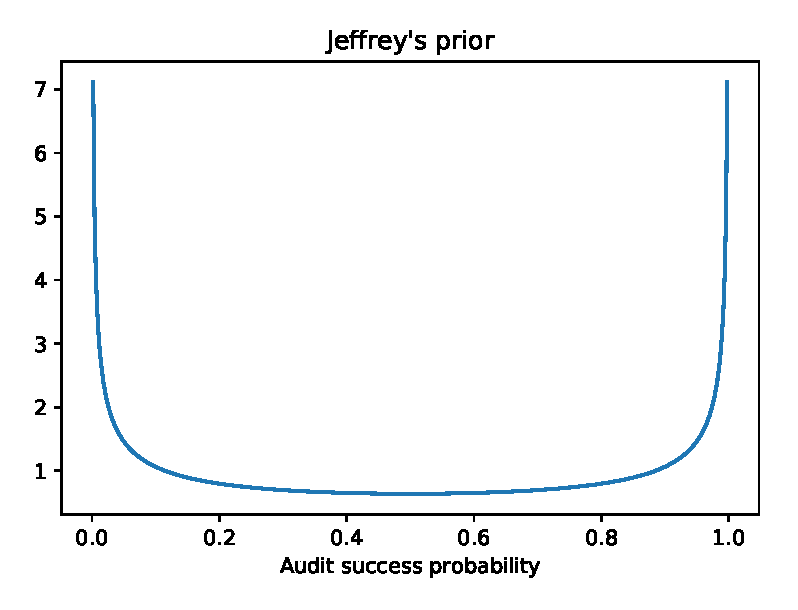
\includegraphics[height=.22\textheight]{audit-success/jeffrey_prior.eps}
    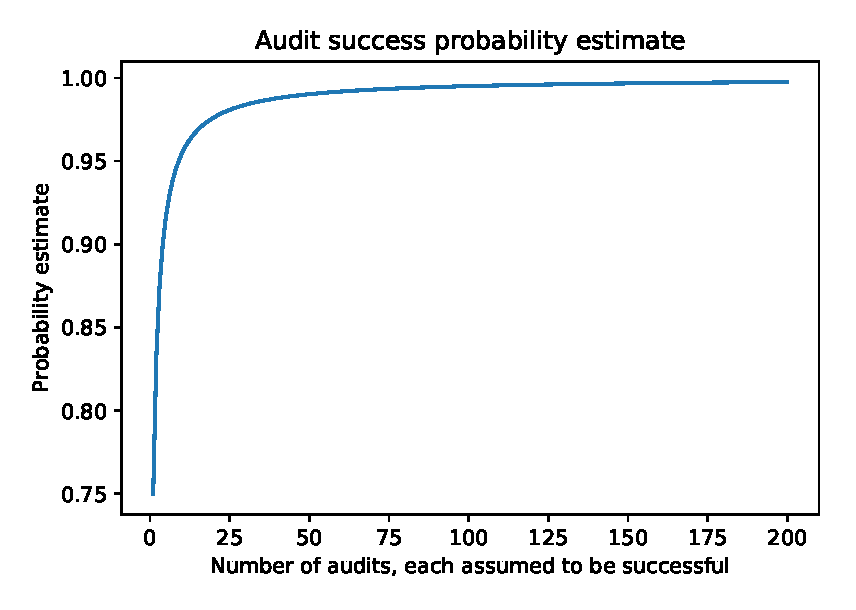
\includegraphics[height=.22\textheight]{audit-success/jeffrey_estimate.eps}
\caption{In Jeffrey's prior, we see the estimate for audit success probability is heavily weighted to be near 0 or near 1.}
\label{fig:jeff_prior}
\end{figure}

\begin{figure}[!htbp]
    \centering
    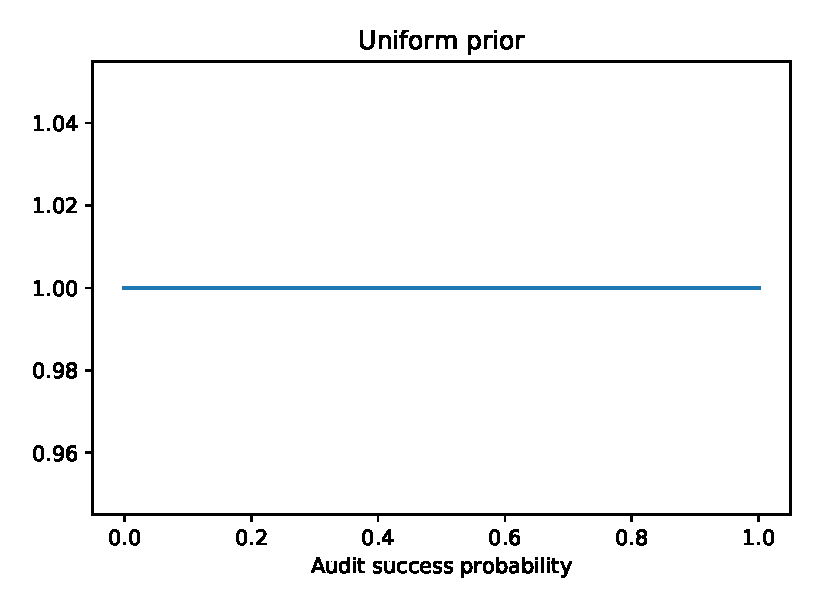
\includegraphics[height=.22\textheight]{audit-success/uniform_prior.eps}
    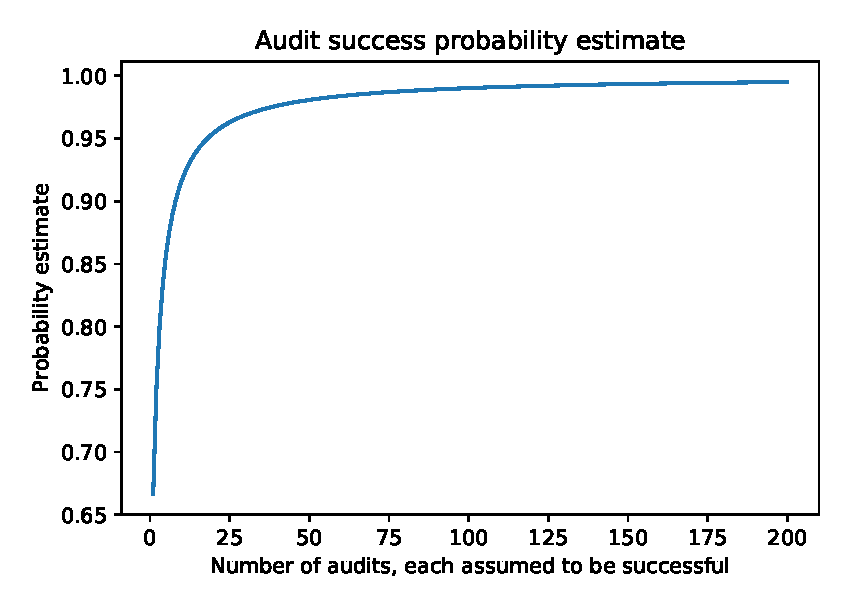
\includegraphics[height=.22\textheight]{audit-success/uniform_estimate.eps}
\caption{Using a Uniform prior, there is no assumption placed on the estimated
audit success probability, and all probabilities are assumed to be equally likely.}
\label{fig:unif_prior}
\end{figure}

We now choose a prior to derive a numerical estimate of the audit success probability
based on the number of audits performed.
There are many reasonable choices of Bayesian priors, but we restrict our attention to
two popular choices: the Uniform prior and Jeffrey's prior \cite{jeffrey}.
Using the Uniform prior $\beta(1,1)$ initializes the experiment
by assigning an equal probability to
all possible outcomes;
that is, the probability of success is drawn from the uniform
distribution on $(0,1)$.
Under Jeffrey's prior $\beta(0.5,0.5)$,
it is assumed that the probability of
success falls towards either extreme, so that a node will return a successful audit
either with probability near 0 or with probability near 1.

\begin{table}[!htbp]
\centering
\begin{tabulary}{\linewidth}{| C | C | C |}\hline
Number of audits & Audit success estimate given uniform prior & Audit success estimate given Jeffrey's prior\\\hline
0 & 0.5 & 0.5 \\
20 & 0.9545 & 0.9762 \\
40 & 0.9762 & 0.9878 \\
80 & 0.9878 & 0.9938 \\
200 & 0.99505 & 0.99751 \\
\hline
\end{tabulary}
\caption{Estimate of audit success probability by
number of audits, each assumed to be successful.
We find that the estimated probability of success begins at 0.5 when there is
no information known about the node (no audits have been performed),
with the estimate quickly jumping to above 99\% in as few as 80 audits using Jeffrey's prior.}
\label{table:audit-success-estimates}
\end{table}

In Table \ref{table:audit-success-estimates},
we present results obtained from using both priors.
We remark that the well-established Bayesian approach
allows us to rapidly gain more confidence
in a node's ability to return a successful audit,
given that the success probability estimate tends closer to 1
with each consecutive audit success.
\FloatBarrier
